% THIS IS SIGPROC-SP.TEX - VERSION 3.1
% WORKS WITH V3.2SP OF ACM_PROC_ARTICLE-SP.CLS
% APRIL 2009
% For tracking purposes - this is V3.1SP - APRIL 2009

\documentclass{acm_proc_article-sp}

% \usepackage[utf8]{inputenc}
% \usepackage[english]{babel} % English language/hyphenation
\usepackage{booktabs}
\usepackage{multicol}
\newcommand{\ra}[1]{\renewcommand{\arraystretch}{#1}}
\usepackage{float}
\usepackage{enumitem}
\usepackage{lipsum}

% references
% \usepackage[autostyle]{csquotes}
\usepackage[
  backend=biber,
  % style=alphabetic,
  citestyle=numeric-comp,
  % citestyle=authoryear,
  natbib=true,
  url=false,
  doi=true,
]{biblatex}
% \bibliography{ref}
\addbibresource{ref.bib}

\begin{document}

\title
{
	Gait Analysis using LSTM%
    \titlenote
    {
        We would like to thank the University of Pittsburgh's Human Movement
        Research Laboratory and its PI, Dr.~Gelsy Torres-Oviedo, for providing
        us with the motion capture data used for the experiments in this paper.
        The collection of these data was approved by the university's
        Institutional Review Board and all participating subjects gave prior
        consent to the use of their data for research purposes.
    }
}


\numberofauthors{3}
\author{
    % 1st. author
    \alignauthor
    Pablo A. Iturralde\\
        \affaddr{Bioengineering Department}\\
        \affaddr{University of Pittsburgh}\\
        \affaddr{Pittsburgh, PA}\\
        \email{pai7@pitt.edu}
    % 2nd. author
    \alignauthor
    Yin Zhong\\
        \affaddr{The Robotics Institute}\\
        \affaddr{Carnegie Mellon University}\\
        \affaddr{Pittsburgh, PA}\\
        \email{yinzhong@andrew.cmu.edu}
    \and
    % 3rd. author
    \alignauthor Jakob Bauer\\
        \affaddr{School of Computer Science}\\
        \affaddr{Carnegie Mellon University}\\
        \affaddr{Pittsburgh, PA}\\
        \email{jsbauer@andrew.cmu.edu}
}

\maketitle

\thispagestyle{empty}

\begin{abstract}
    \lipsum[1-2]
\end{abstract}

% \category{J.3}
% {Life and Medical Sciences}
% {Biology and genetics}
% \terms{ACM proceedings, \LaTeX, text tagging}
% \keywords{Gait event, Heel strike, Toe off, LSTM}

\vskip 12em

\section{Introduction}
\label{sec:Introduction}

In order to study human gait,
it is necessary to divide the gait cycle into swing phase and stance phase.
The transition between the phases is marked by two events:
the subject's heel hitting the ground (heel strike) and the subject's toe
lifting off the ground (toe off).
It is paramount to accurately identify these events because otherwise, no
meaningful comparison of different stride cycles is possible.

% TODO introduce motion capture data

There are three basic approaches to event detection.
The first approach uses visual inspection to manually label the events.
Although quite accurate, the cost associated with this method is prohibitive for
all but the smallest amounts of data.
For this reason, it is not usually used as a stand-alone method but rather as a
postprocessing step for automated event detection systems or as a means to
generate small sets of hand-labeled test data.
The second approach uses dedicated hardware such as force plates that measure
ground reaction forces and foot switches that are pressed when the foot is in
contact with the ground.
Due to its high accuracy, hardware-based methods are considered to be
state of the art for gait event identification.
However, their usefulness is limited by the fact that many laboratories do not
have access to the necessary equipment.
Furthermore, there is a risk of affecting the gait because some of the devices
require the modification of normal footware.
The third approach consists in automatated event detection based on solely on
the data.
If succesful, this approach is superior to the other two because it scales
easily, does not require additional equipment and does not pose a risk of
affecting the gait.

Given these apparent advatages, it is not surprising that several data-based
methods have been proposed in the literature.
Although some of those methods achieve results that are accurate enough to be
useful in practice, they also have drawbacks such as relying heavily on
questionable heuristics or requiring an undue amount of data preprocessing.
For this reason, we present a new approach to gait event detection using a
Long Short-Term Memory (LSTM) recurrent neural network (RNN).
We believe that our method is superior to existing approaches both in terms of
accuracy and in terms of only requirying a small amount of training data and
preprocessing.

This paper is organized as follows:
Section~\ref{sec:Previous Work}
discusses some of the existing data-based methods for event detection;
Section~\ref{sec:LSTM}
gives a short overview over LSTM networks in general;
Section~\ref{sec:Data}
contains a description the dataset;
Sections~\ref{sec:Network Architecture} and \ref{sec:Network Training}
describe the architecture and training of our network;
Section~\ref{sec:Results}
presents the experimental results and compares them to existing baselines;
Section~\ref{sec:Conclusion and Future Work}
concludes and shows possible paths for future work.

\section{Previous Work}
\label{sec:Previous Work}

% \subsection{Heuristic Approach}
% \label{sub:Heuristic Approach}
\subsection{Foot Velocity Algorithm}
\label{sub:Foot Velocity Algorithm}

The Foot Velocity Algorithm (FVA) proposed by
\citet{Oconnor2007}
belongs to a category of algorithms that use heuristics such as the velocity
and acceleration of heel and toe markers to detect motion events.
There are other examples of such algorithms, notably the one developped by
\citet{Hreljac2000}.
These algorithms are quite similar, we will therefore restrict the discussion
to the FVA.

The FVA takes as its input the location of the heel and toe markers as a
function of time.
After passing the data through a simple low pass filter,
a new virtual marker representing the foot center is created by taking the mean
of the heel and toe markers.
Finally, the velocity of this virtual marker is calculated.
Due to the quasi-periodic nature of walking, the graph of the velocity signal
exhibits a repeating pattern in which the toe off event is marked by a global
maximum and the heel strike by a local minimum.
This makes it possible to first detect the toe off event for each cycle and
then, in a second step, go through all the possible candidates for the heel
strike.
By using a constraint on the heel strike time, one of the candidates is selected
as the heel strike event.

The FVA is easy to implement as it does not require preprocessing beyond simple
signal processing and because it does not require any training.
This makes it a popular choice in practice.
That said, the FVA has several problems.
First, it makes questionable assumptions about the relationship between the 
marker location and the gait cycle.
For instance, it is not clear that the marker velocity peaks exactly coincide
with the events to be identified.
Secondly, the algorithm is very sensitive to a threshold that has to be applied 
in order to restrict the search for heel strike candidates.
The value of this threshold has to be manually tuned for each subject and, if
not chosen correctly, the algorithm fails catastrophically.
Finally, the accuracy of FVA is bad when compared to more sophisticated methods
such as neural network and LSTM
(cf. Section~\ref{sec:Results}).

% TODO problem with pathological gaits

\subsection{Neural Network}
\label{sub:Neural Network}

description

preprocessing (dimensionality reduction)

baseline2

\section{LSTM}
\label{sec:LSTM}

\section{Data}
\label{sec:Data}

\section{Network Architecture}
\label{sec:Network Architecture}

\section{Network Training}
\label{sec:Network Training}

\section{Results}
\label{sec:Results}

\section{Conclusion and Future Work}
\label{sec:Conclusion and Future Work}


% \section{Data}
% For the initial training purposes, we selected data from 8 healthy subjects walking in a treadmill at three different speeds for 100 seconds each. Additionally, we took data from 13 stroke subjects, walking at a single speed for 100 seconds. For each subject, the input data is 3D marker position of 18 different markers placed in the same anatomical positions for each subject, sampled at 100Hz. The event labels (target) were computed from ground force reaction data samples at 1kHz for healthy subjects, and 2kHz for stroke subjects. This is currently considered the gold standard \cite{miller_gait_2009,miller_gait_2009,Hreljac2000}. \\
% %The problem is then to classify each sample in time as one of four different classes: both feet in contact with the ground, both feet off the ground, left feet only on the ground and right feet only on the ground.
% \section{Algorithms}
%
% In order to compare our results, we implemented two algorithms presented in the literature: a heuristic-based method \cite{oconnor_automatic_2007}, and a neural-network approach \cite{miller_gait_2009}.
%
% \subsection{O'Connor's Heuristic}
% \citet{oconnor_automatic_2007} describe a heuristic to compute gait events by just considering vertical and horizontal speed of heel and toe markers respectively, and using a peak detection algorithm.
%
% \subsection{Miller's Neural Network}
% \citet{miller_gait_2009} is one of the few data-driven efforts of event estimation. It uses a classical NN to classify each sample. The inputs are computed from the position, instantaneous velocity and instantaneous acceleration of each available motion-capture marker in a time-window centered around the desired time sample. Because the inputs are too many (the total input size grows linearly with the window size and the number of markers), a dimensionality reduction technique (PCA) is used before training the NN.
%
% \subsection{Our approach: Long Short Term Memory Neural Network}
% %\vspace{-1cm}
%
% Gait event detection is a form of \textit{sequence labeling}, i.e., assigning a sequence of labels to a sequence of data.
% One approach to sequence labeling is the use of recurrent neural networks (RNN). However, due to the vanishing gradient problem RNNs cannot store information for a long time which means that their usefulness for sequence labeling is limited.
% One solution to this problem is the use of a Long Short-Term Memory (LSTM) architecture instead of conventional RNNs \cite{graves_supervised_2012}.
% In LSTM, the summation units in the hidden layer are replaced with so-called memory blocks.
% These blocks consist of a memory cell as well as three multiplicative units called input gate, output gate and forget gate.
% The gates allow information to be stored in the memory cell for long periods of time.
% While we haven't decided on the overall design of our LSTM network yet, it will probably have specifications along the lines of:
% \begin{itemize}[noitemsep,nolistsep]
% \item Up to 54 input units that each take the sequence corresponding to one marker as input; the reason we might not need all 54 marker sequences is that some of the markers (e.g., for the hip) presumably carry little useful information.
% \item A hidden layer of LSTM memory blocks; the exact number will depend on the number of input units.
% \item 2 output units (one for each leg); the output will be thresholded with '0' corresponding to stance phase and '1' corresponding to swing phase.
% \end{itemize}
%
% \section{Computational Resources}
%
% For the LSTM network we are using
% an Amazon EC2 instance of type g2.2xlarge.
% This instance type comes with an 8 core 2.6 GHz Intel Xeon E5-2670 processor and an Nvidia GRID K520 GPU that is composed of two 4 GB GK104 GPUs.
% We chose Torch as our computing framework.
%
% \section{Intermediate Results}
% We implemented and tested the two methods described in \cite{oconnor_automatic_2007} and \cite{miller_gait_2009}. Results are in line with the ones presented on each paper. Summaries of the true error (detected event time minus actual event time) can be found in Figures~\ref{fig:oconner} and \ref{fig:miller}.
% There are no results yet for the LSTM approach.
%
% \section{Difficulties and Future Work}
% In the following weeks we will be implementing an LSTM network on Torch. As we have no experience using Torch in the past, we are not sure how long it will take.\\
%
% Other future work includes feature engineering to determine the most relevant input variables, from all the available marker position data and its derivatives, in order to reduce the size of the network that has to be trained. We would also like to extend the capabilities of the method to data that was acquired in natural walking (as opposed to treadmill walking). We believe adequate feature engineering may be enough to achieve this objective too.\\

\printbibliography

% \begin{figure*}
% \begin{center}
% 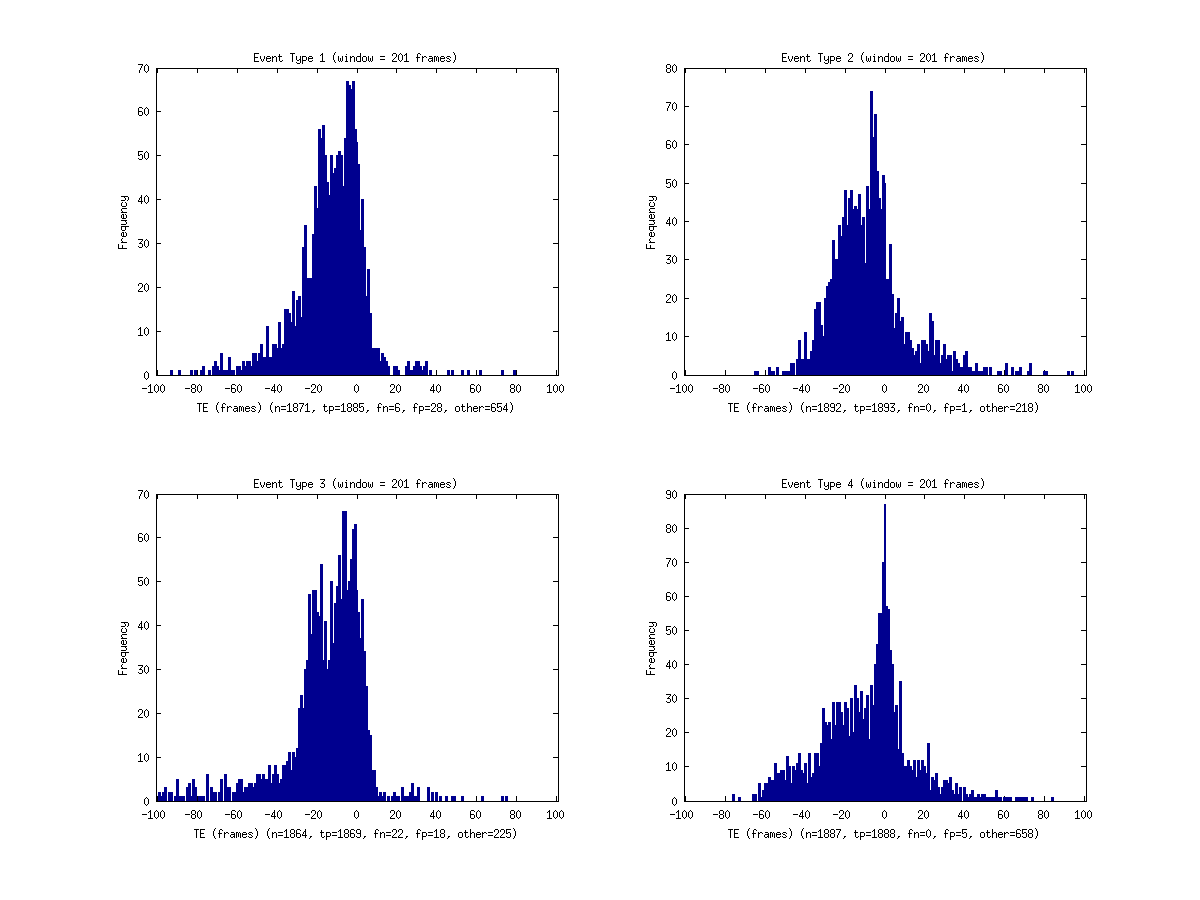
\includegraphics[width=0.70\textwidth]{figures/trueErrorsPerEventType_oconner.png}
% \end{center}
% \caption{
% True errors per event type for O'Connor's heuristic.
% The data set consists of 8 subjects à 3 trials each.
% The panes are (clockwise starting from the top-left):
% Left Heel Strike, Right Toe Off, Right Heel Strike, Left Toe Off.
% One frame corresponds to 1 ms.
% If the estimated event was not within 100 frames from the true event then it is reported as "other" and not shown in the histogram.
% }
% \label{fig:oconner}
% \end{figure*}
%
% \begin{figure*}[t]
% \begin{center}
% 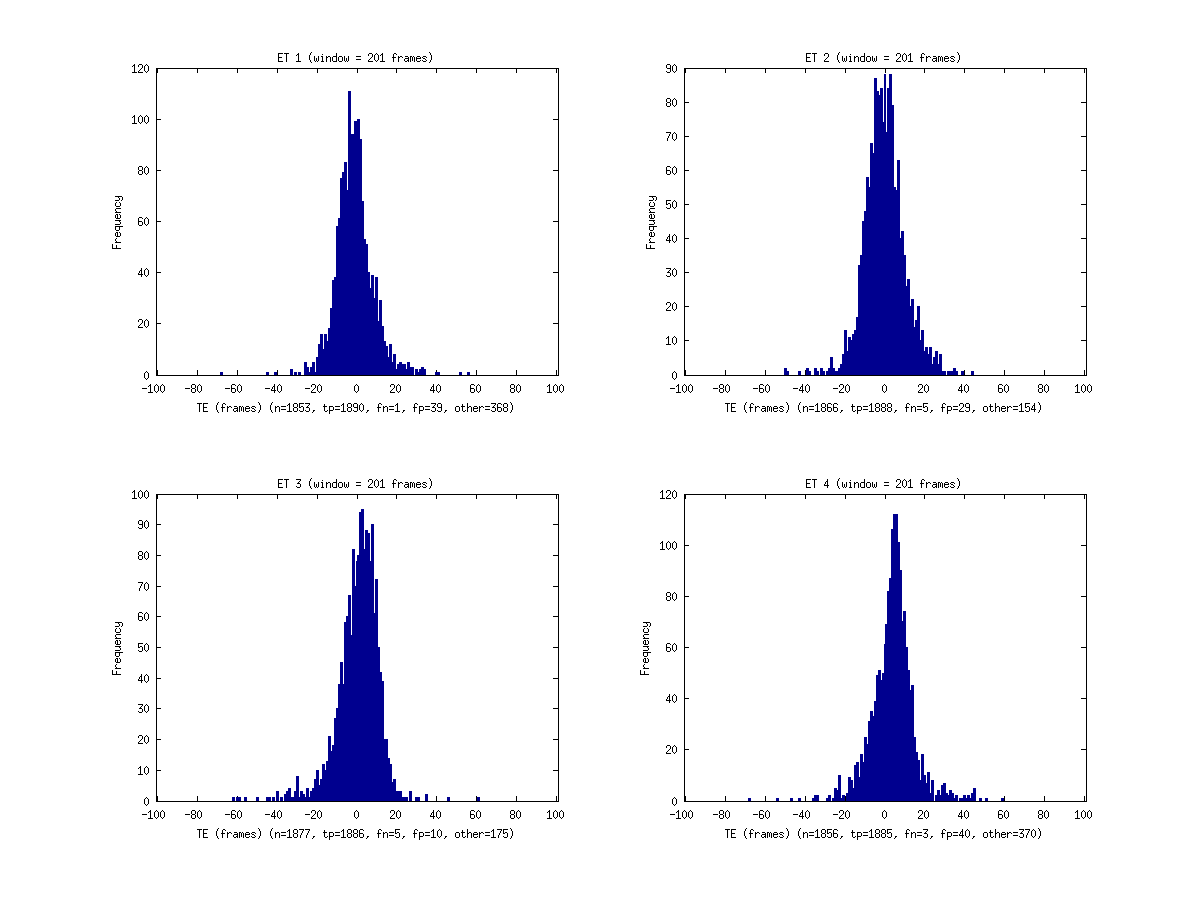
\includegraphics[width=0.70\textwidth]{figures/trueErrorsPerEventType_miller.png}
% \end{center}
% \caption{
% True errors per event type for Miller's neural network.
% The data set consists of 8 subjects à 3 trials each.
% The panes are (clockwise starting from the top-left):
% Left Heel Strike, Right Toe Off, Right Heel Strike, Left Toe Off.
% One frame corresponds to 0.5 ms.
% If the estimated event was not within 100 frames from the true event then it is reported as "other" and not shown in the histogram.
% }
% \label{fig:miller}
% \end{figure*}

% \bibliographystyle{abbrv}
% \bibliographystyle{plain}

% \appendix

\end{document}
